% Options for packages loaded elsewhere
\PassOptionsToPackage{unicode}{hyperref}
\PassOptionsToPackage{hyphens}{url}
%
\documentclass[
]{book}
\usepackage{amsmath,amssymb}
\usepackage{iftex}
\ifPDFTeX
  \usepackage[T1]{fontenc}
  \usepackage[utf8]{inputenc}
  \usepackage{textcomp} % provide euro and other symbols
\else % if luatex or xetex
  \usepackage{unicode-math} % this also loads fontspec
  \defaultfontfeatures{Scale=MatchLowercase}
  \defaultfontfeatures[\rmfamily]{Ligatures=TeX,Scale=1}
\fi
\usepackage{lmodern}
\ifPDFTeX\else
  % xetex/luatex font selection
\fi
% Use upquote if available, for straight quotes in verbatim environments
\IfFileExists{upquote.sty}{\usepackage{upquote}}{}
\IfFileExists{microtype.sty}{% use microtype if available
  \usepackage[]{microtype}
  \UseMicrotypeSet[protrusion]{basicmath} % disable protrusion for tt fonts
}{}
\makeatletter
\@ifundefined{KOMAClassName}{% if non-KOMA class
  \IfFileExists{parskip.sty}{%
    \usepackage{parskip}
  }{% else
    \setlength{\parindent}{0pt}
    \setlength{\parskip}{6pt plus 2pt minus 1pt}}
}{% if KOMA class
  \KOMAoptions{parskip=half}}
\makeatother
\usepackage{xcolor}
\usepackage{color}
\usepackage{fancyvrb}
\newcommand{\VerbBar}{|}
\newcommand{\VERB}{\Verb[commandchars=\\\{\}]}
\DefineVerbatimEnvironment{Highlighting}{Verbatim}{commandchars=\\\{\}}
% Add ',fontsize=\small' for more characters per line
\usepackage{framed}
\definecolor{shadecolor}{RGB}{248,248,248}
\newenvironment{Shaded}{\begin{snugshade}}{\end{snugshade}}
\newcommand{\AlertTok}[1]{\textcolor[rgb]{0.94,0.16,0.16}{#1}}
\newcommand{\AnnotationTok}[1]{\textcolor[rgb]{0.56,0.35,0.01}{\textbf{\textit{#1}}}}
\newcommand{\AttributeTok}[1]{\textcolor[rgb]{0.13,0.29,0.53}{#1}}
\newcommand{\BaseNTok}[1]{\textcolor[rgb]{0.00,0.00,0.81}{#1}}
\newcommand{\BuiltInTok}[1]{#1}
\newcommand{\CharTok}[1]{\textcolor[rgb]{0.31,0.60,0.02}{#1}}
\newcommand{\CommentTok}[1]{\textcolor[rgb]{0.56,0.35,0.01}{\textit{#1}}}
\newcommand{\CommentVarTok}[1]{\textcolor[rgb]{0.56,0.35,0.01}{\textbf{\textit{#1}}}}
\newcommand{\ConstantTok}[1]{\textcolor[rgb]{0.56,0.35,0.01}{#1}}
\newcommand{\ControlFlowTok}[1]{\textcolor[rgb]{0.13,0.29,0.53}{\textbf{#1}}}
\newcommand{\DataTypeTok}[1]{\textcolor[rgb]{0.13,0.29,0.53}{#1}}
\newcommand{\DecValTok}[1]{\textcolor[rgb]{0.00,0.00,0.81}{#1}}
\newcommand{\DocumentationTok}[1]{\textcolor[rgb]{0.56,0.35,0.01}{\textbf{\textit{#1}}}}
\newcommand{\ErrorTok}[1]{\textcolor[rgb]{0.64,0.00,0.00}{\textbf{#1}}}
\newcommand{\ExtensionTok}[1]{#1}
\newcommand{\FloatTok}[1]{\textcolor[rgb]{0.00,0.00,0.81}{#1}}
\newcommand{\FunctionTok}[1]{\textcolor[rgb]{0.13,0.29,0.53}{\textbf{#1}}}
\newcommand{\ImportTok}[1]{#1}
\newcommand{\InformationTok}[1]{\textcolor[rgb]{0.56,0.35,0.01}{\textbf{\textit{#1}}}}
\newcommand{\KeywordTok}[1]{\textcolor[rgb]{0.13,0.29,0.53}{\textbf{#1}}}
\newcommand{\NormalTok}[1]{#1}
\newcommand{\OperatorTok}[1]{\textcolor[rgb]{0.81,0.36,0.00}{\textbf{#1}}}
\newcommand{\OtherTok}[1]{\textcolor[rgb]{0.56,0.35,0.01}{#1}}
\newcommand{\PreprocessorTok}[1]{\textcolor[rgb]{0.56,0.35,0.01}{\textit{#1}}}
\newcommand{\RegionMarkerTok}[1]{#1}
\newcommand{\SpecialCharTok}[1]{\textcolor[rgb]{0.81,0.36,0.00}{\textbf{#1}}}
\newcommand{\SpecialStringTok}[1]{\textcolor[rgb]{0.31,0.60,0.02}{#1}}
\newcommand{\StringTok}[1]{\textcolor[rgb]{0.31,0.60,0.02}{#1}}
\newcommand{\VariableTok}[1]{\textcolor[rgb]{0.00,0.00,0.00}{#1}}
\newcommand{\VerbatimStringTok}[1]{\textcolor[rgb]{0.31,0.60,0.02}{#1}}
\newcommand{\WarningTok}[1]{\textcolor[rgb]{0.56,0.35,0.01}{\textbf{\textit{#1}}}}
\usepackage{longtable,booktabs,array}
\usepackage{calc} % for calculating minipage widths
% Correct order of tables after \paragraph or \subparagraph
\usepackage{etoolbox}
\makeatletter
\patchcmd\longtable{\par}{\if@noskipsec\mbox{}\fi\par}{}{}
\makeatother
% Allow footnotes in longtable head/foot
\IfFileExists{footnotehyper.sty}{\usepackage{footnotehyper}}{\usepackage{footnote}}
\makesavenoteenv{longtable}
\usepackage{graphicx}
\makeatletter
\newsavebox\pandoc@box
\newcommand*\pandocbounded[1]{% scales image to fit in text height/width
  \sbox\pandoc@box{#1}%
  \Gscale@div\@tempa{\textheight}{\dimexpr\ht\pandoc@box+\dp\pandoc@box\relax}%
  \Gscale@div\@tempb{\linewidth}{\wd\pandoc@box}%
  \ifdim\@tempb\p@<\@tempa\p@\let\@tempa\@tempb\fi% select the smaller of both
  \ifdim\@tempa\p@<\p@\scalebox{\@tempa}{\usebox\pandoc@box}%
  \else\usebox{\pandoc@box}%
  \fi%
}
% Set default figure placement to htbp
\def\fps@figure{htbp}
\makeatother
\setlength{\emergencystretch}{3em} % prevent overfull lines
\providecommand{\tightlist}{%
  \setlength{\itemsep}{0pt}\setlength{\parskip}{0pt}}
\setcounter{secnumdepth}{5}
\usepackage{booktabs}
\usepackage[]{natbib}
\bibliographystyle{plainnat}
\usepackage{bookmark}
\IfFileExists{xurl.sty}{\usepackage{xurl}}{} % add URL line breaks if available
\urlstyle{same}
\hypersetup{
  pdftitle={A Minimal Book Example},
  pdfauthor={John Doe},
  hidelinks,
  pdfcreator={LaTeX via pandoc}}

\title{A Minimal Book Example}
\author{John Doe}
\date{2025-03-27}

\begin{document}
\maketitle

{
\setcounter{tocdepth}{1}
\tableofcontents
}
\chapter{About}\label{about}

This is a \emph{sample} book written in \textbf{Markdown}. You can use anything that Pandoc's Markdown supports; for example, a math equation \(a^2 + b^2 = c^2\).

\section{Usage}\label{usage}

Each \textbf{bookdown} chapter is an .Rmd file, and each .Rmd file can contain one (and only one) chapter. A chapter \emph{must} start with a first-level heading: \texttt{\#\ A\ good\ chapter}, and can contain one (and only one) first-level heading.

Use second-level and higher headings within chapters like: \texttt{\#\#\ A\ short\ section} or \texttt{\#\#\#\ An\ even\ shorter\ section}.

The \texttt{index.Rmd} file is required, and is also your first book chapter. It will be the homepage when you render the book.

\section{Render book}\label{render-book}

You can render the HTML version of this example book without changing anything:

\begin{enumerate}
\def\labelenumi{\arabic{enumi}.}
\item
  Find the \textbf{Build} pane in the RStudio IDE, and
\item
  Click on \textbf{Build Book}, then select your output format, or select ``All formats'' if you'd like to use multiple formats from the same book source files.
\end{enumerate}

Or build the book from the R console:

\begin{Shaded}
\begin{Highlighting}[]
\NormalTok{bookdown}\SpecialCharTok{::}\FunctionTok{render\_book}\NormalTok{()}
\end{Highlighting}
\end{Shaded}

To render this example to PDF as a \texttt{bookdown::pdf\_book}, you'll need to install XeLaTeX. You are recommended to install TinyTeX (which includes XeLaTeX): \url{https://yihui.org/tinytex/}.

\section{Preview book}\label{preview-book}

As you work, you may start a local server to live preview this HTML book. This preview will update as you edit the book when you save individual .Rmd files. You can start the server in a work session by using the RStudio add-in ``Preview book'', or from the R console:

\begin{Shaded}
\begin{Highlighting}[]
\NormalTok{bookdown}\SpecialCharTok{::}\FunctionTok{serve\_book}\NormalTok{()}
\end{Highlighting}
\end{Shaded}

\chapter{Rstudio}\label{rstudio}

\textbf{Rstudio shortcuts}

\begin{longtable}[]{@{}
  >{\raggedright\arraybackslash}p{(\linewidth - 2\tabcolsep) * \real{0.4783}}
  >{\raggedright\arraybackslash}p{(\linewidth - 2\tabcolsep) * \real{0.5217}}@{}}
\toprule\noalign{}
\begin{minipage}[b]{\linewidth}\raggedright
keyboard combination
\end{minipage} & \begin{minipage}[b]{\linewidth}\raggedright
function
\end{minipage} \\
\midrule\noalign{}
\endhead
\bottomrule\noalign{}
\endlastfoot
opt + \_ & insert assignment operator \texttt{\textless{}-} \\
ESC or ctrl + C & exit \texttt{+} prompt \\
ctrl + shift + m & add pipe operator ``\%\textgreater\%'' \\
{ctrl + \texttt{{[}}/\texttt{{]}} } & indent or unindent \\
cmd + D & delete one row \\
cmd + 1 & move cursor to console window \\
cmd + 2 & move cursor to editor window \\
ctrl + shift + S & add 80 hyphens \texttt{-\/-\/-} to signal a new chapter (Addin) \\
ctrl + shift + = & add 80 equals \texttt{===} to signal a new Chapter (Addin) \\
shift + cmd +N & new R script \\
cmd + \(\uparrow\) / \(\downarrow\) & in console, get a list of command history \\
shift + \(\uparrow\) / \(\downarrow\) & select one line up/down \\
fn + F2 & \texttt{view()} an object, don't select the object \\
cmd + shift + 1 & activate X11() window \\
{ctrl (+ shift) + tab} & next (last) tab in scriptor (this applies to all apps); hit ctrl first, then shift if necessary, last tab \\
\end{longtable}

{\textbf{Source}}

\begin{longtable}[]{@{}
  >{\raggedright\arraybackslash}p{(\linewidth - 2\tabcolsep) * \real{0.2817}}
  >{\raggedright\arraybackslash}p{(\linewidth - 2\tabcolsep) * \real{0.7183}}@{}}
\toprule\noalign{}
\begin{minipage}[b]{\linewidth}\raggedright
keyboard combination
\end{minipage} & \begin{minipage}[b]{\linewidth}\raggedright
function
\end{minipage} \\
\midrule\noalign{}
\endhead
\bottomrule\noalign{}
\endlastfoot
cmd + return & Run current line/selection \\
opt + return & Run current line/selection (retain cursor position) \\
\end{longtable}

{\textbf{\texttt{Rmd} related}}

\begin{longtable}[]{@{}
  >{\raggedright\arraybackslash}p{(\linewidth - 2\tabcolsep) * \real{0.2500}}
  >{\raggedright\arraybackslash}p{(\linewidth - 2\tabcolsep) * \real{0.7500}}@{}}
\toprule\noalign{}
\begin{minipage}[b]{\linewidth}\raggedright
keyboard combination
\end{minipage} & \begin{minipage}[b]{\linewidth}\raggedright
function
\end{minipage} \\
\midrule\noalign{}
\endhead
\bottomrule\noalign{}
\endlastfoot
cmd + shift + K & \textbf{Knit} rmd \\
cmd + opt + C & run current code chunk in \texttt{Rmd} \\
cmd + opt + I & insert code chunks in \texttt{Rmd}, i.e., \texttt{\textasciigrave{}\textasciigrave{}\textasciigrave{}\{r\}} and \texttt{\textasciigrave{}\textasciigrave{}\textasciigrave{}} \\
\end{longtable}

Q: How to print output in console rather than inline in Rmd?

A: Choose the gear in the editor toolbar and choose ``Chunk Output in Console''.

{\textbf{Set working directory}}

\begin{Shaded}
\begin{Highlighting}[]
\NormalTok{dir\_folder }\OtherTok{\textless{}{-}} \FunctionTok{dirname}\NormalTok{(rstudioapi}\SpecialCharTok{::}\FunctionTok{getSourceEditorContext}\NormalTok{()}\SpecialCharTok{$}\NormalTok{path) }\CommentTok{\# get the dir name of the current script}
\FunctionTok{setwd}\NormalTok{(dir\_folder) }\CommentTok{\# set as working dir}
\end{Highlighting}
\end{Shaded}

RStudio projects are associated with R working directories. You can create an RStudio project:

\begin{itemize}
\tightlist
\item
  In a brand new directory
\item
  In an existing directory where you already have R code and data
\item
  By cloning a version control (Git or Subversion) repository
\end{itemize}

Why using R projects:

\begin{enumerate}
\def\labelenumi{\arabic{enumi}.}
\tightlist
\item
  I don't need to use \texttt{setwd} at the start of each script, and if I move the base project folder it will still work.
\item
  I have a personal package with a custom project, which creates my folders just the way I like them. This makes it so that the basic locations for data, outputs and analysis is the same across my work.
\end{enumerate}

Double-click on a \texttt{.Rproj} file to open a fresh instance of RStudio, with the working directory and file browser pointed at the project folder.

Q: What is an \textbf{R session}? And when do I use it?

A: Multiple concurrent sessions can be useful when you want to:

\begin{itemize}
\tightlist
\item
  Run multiple analyses in parallel
\item
  Keep multiple sessions open indefinitely
\item
  Participate in one or more \href{https://support.posit.co/hc/en-us/articles/211659737}{shared projects}
\end{itemize}

\textbf{Launch a new project-less RStudio session}

\begin{Shaded}
\begin{Highlighting}[]
\CommentTok{\# run in console}
\NormalTok{rstudioapi}\SpecialCharTok{::}\FunctionTok{terminalExecute}\NormalTok{(}\StringTok{"open {-}n /Applications/RStudio.app"}\NormalTok{, }\AttributeTok{show =} \ConstantTok{FALSE}\NormalTok{)}
\end{Highlighting}
\end{Shaded}

\texttt{-n} Open a new instance of the application(s) even if one is already running.

\texttt{rstudioapi::terminalExecute(command,\ workingDir\ =\ NULL,\ env\ =\ character(),\ show\ =\ TRUE)} tells R to run the system command in quotes.

\begin{itemize}
\tightlist
\item
  \texttt{command} System command to be invoked, as a character string.
\item
  \texttt{workingDir} Working directory for command
\item
  \texttt{env} Vector of name=value strings to set environment variables
\item
  \texttt{show} If FALSE, terminal won't be brought to front
\end{itemize}

The {\texttt{rstudioapi}} package provides an interface for interacting with the RStudio IDE with R code. Using\texttt{rstudioapi}, you can:

\begin{itemize}
\tightlist
\item
  Examine, manipulate, and save the contents of documents currently open in RStudio,
\item
  Create, open, or re-open RStudio projects,
\item
  Prompt the user with different kinds of dialogs (e.g.~for selecting a file or folder, or requesting a password from the user),
\item
  Interact with RStudio terminals,
\item
  Interact with the R session associated with the current RStudio instance.
\end{itemize}

\begin{center}\rule{0.5\linewidth}{0.5pt}\end{center}

\textbf{Set up Development Tools}

\url{https://cran.r-project.org/bin/macosx/tools/}

\begin{itemize}
\item
  install Xcode command line tools

\begin{Shaded}
\begin{Highlighting}[]
\FunctionTok{sudo}\NormalTok{ xcode{-}select }\AttributeTok{{-}{-}install}
\end{Highlighting}
\end{Shaded}
\item
  install GNU Fortran compiler

  Using \textbf{Apple silicon} (aka arm64, aarch64, M1) Macs Fortran compiler
\item
  Go to \url{https://www.xquartz.org/}, download the .dmg and run the installer.
\item
  Verify that build tools are installed and available by opening an R console and running

\begin{Shaded}
\begin{Highlighting}[]
\FunctionTok{install.packages}\NormalTok{(}\StringTok{"pkgbuild"}\NormalTok{)}
\NormalTok{pkgbuild}\SpecialCharTok{::}\FunctionTok{check\_build\_tools}\NormalTok{()}
\end{Highlighting}
\end{Shaded}
\end{itemize}

\begin{center}\rule{0.5\linewidth}{0.5pt}\end{center}

\textbf{Insert Code Session}

To insert a new code section you can use the \textbf{Code} -\textgreater{} \textbf{Insert Section} command. Alternatively, any comment line which includes at least four trailing dashes (\texttt{-}), equal signs (\texttt{=}), or pound signs (\texttt{\#}) automatically creates a code section.

\textbf{Define your own shortcuts}

\url{https://www.statworx.com/ch/blog/defining-your-own-shortcut-in-rstudio/}

\url{https://www.r-bloggers.com/2020/03/defining-your-own-shortcut-in-rstudio/}

Install the shortcut packages.

Add code session separators, \texttt{-\/-\/-} or \texttt{===}.

\begin{Shaded}
\begin{Highlighting}[]
\FunctionTok{install.packages}\NormalTok{(}
    \CommentTok{\# same path as above}
  \StringTok{"\textasciitilde{}/Downloads/shoRtcut\_0.1.0.tar.gz"}\NormalTok{, }
  \CommentTok{\# indicate it is a local file}
  \AttributeTok{repos =} \ConstantTok{NULL}\NormalTok{)}
\FunctionTok{install.packages}\NormalTok{(}
    \CommentTok{\# same path as above}
  \StringTok{"\textasciitilde{}/Downloads/shoRtcut2\_0.1.0.tar.gz"}\NormalTok{, }
  \CommentTok{\# indicate it is a local file}
  \AttributeTok{repos =} \ConstantTok{NULL}\NormalTok{)}
\end{Highlighting}
\end{Shaded}

Now go to Tools \textgreater{} Modify Keyboard Shortcuts and search for ``dashes''. Here you can define the keyboard combination by clicking inside the empty Shortcut field and pressing the desired key-combination on your keyboard. Click Apply, and that's it!

\begin{center}\rule{0.5\linewidth}{0.5pt}\end{center}

\section{Dark Theme}\label{dark-theme}

\url{https://community.rstudio.com/t/fvaleature-req-word-background-highlight-color-in-find-and-spellcheck/18578/3}

\url{https://rstudio.github.io/rstudio-extensions/rstudio-theme-creation.html}

\url{https://docs.posit.co/ide/user/ide/guide/ui/appearance.html\#creating-custom-themes-for-rstudio}

\texttt{.ace\_marker-layer\ .ace\_selection} Changes the color and style of the highlighting for the currently selected line or block of lines.

\texttt{.ace\_marker-layer\ .ace\_bracket} Changes the color and style of the highlighting on matching brackets.

\textbf{Recommended highlight color}: \texttt{rgba(255,\ 0,\ 0,\ 0.47)}

\texttt{RStudio} editor theme directory on Mac:

right click \texttt{RStudio.app}, ``Show Package Contents'' to navigate to the application folder.

\texttt{/Applications/RStudio.app/Contents/Resources/resources/themes/ambiance.rstheme}

Custom theme (user-defined) folder:

\begin{itemize}
\tightlist
\item
  \texttt{\textasciitilde{}/.config/rstudio/themes/idle\_fingers\_2.rstheme} on mac
\item
  \href{https://github.com/z3tt/viridis-theme/blob/main/viridis.rstheme}{viridis-theme}
\end{itemize}

\begin{Shaded}
\begin{Highlighting}[]
\CommentTok{/* yaml tag */}
\FunctionTok{.ace\_meta.ace\_tag}\NormalTok{ \{}
  \KeywordTok{color}\CharTok{:} \ConstantTok{\#2499DA}\OperatorTok{;}
\NormalTok{\}}
\CommentTok{/* quoted by $...$ and code chunk options */}
\FunctionTok{.ace\_support.ace\_function}\NormalTok{ \{}
  \KeywordTok{color}\CharTok{:} \ConstantTok{\#55C667}\OperatorTok{;}
\NormalTok{\}}
\end{Highlighting}
\end{Shaded}

\begin{center}\rule{0.5\linewidth}{0.5pt}\end{center}

\section{Update R}\label{update-r}

Q: How to tell which version of R you are running?\\
A: In the R terminal, type \texttt{R.version}.

The key thing to be aware of is that when you update R, {if you just download the latest version from the website, you will lose all your packages!} ❌

The easiest way to update R and not cause yourself a huge headache is to use the \texttt{installr} package. When you use the \texttt{updateR()} function, a series of dialogue boxes will appear. These should be fairly self-explanatory but there is a \href{https://www.r-statistics.com/2015/06/a-step-by-step-screenshots-tutorial-for-upgrading-r-on-windows/\#google_vignette}{full step-by-step guide} available for how to use \texttt{installr}, the important bit is to {select ``Yes'' when it asked if you would like to copy your packages from the older version of R}.

\begin{Shaded}
\begin{Highlighting}[]
\CommentTok{\# Install the installr package}
\FunctionTok{install.packages}\NormalTok{(}\StringTok{"installr"}\NormalTok{)}

\CommentTok{\# Load installr}
\FunctionTok{library}\NormalTok{(installr)}

\CommentTok{\# Run the update function}
\FunctionTok{updateR}\NormalTok{()}
\end{Highlighting}
\end{Shaded}

\begin{center}\rule{0.5\linewidth}{0.5pt}\end{center}

\section{Packages Management}\label{packages-management}

\textbf{Load packages}

Q: What is the difference btw \texttt{library(package)} and \texttt{require(package)}?\\
A:

\begin{itemize}
\item
  \texttt{library(package)} returns an error if the package doesn't exist.
\item
  \texttt{require(package)} returns \texttt{FALSE} if the package is not found and \texttt{TRUE} if the packages is loaded. \texttt{require} is designed for use inside other functions, such as using the value it returns in some error checking loop, as it outputs a warning and continues if the package is not found.
\end{itemize}

Q: How to reload a package after updating?\\
A: Call \texttt{detach(package:pkg,\ unload\ =\ TRUE)} or \texttt{unloadNamespace} first, then use \texttt{library(pkg)} to reload. If you use \texttt{library} on a package whose namespace is loaded, it attaches the exports of the already loaded namespace. So detaching and re-attaching a package may not refresh some or all components of the package, and is inadvisable. The most reliable way to completely detach a package is to {restart R}.

For example, if we want to detach \texttt{ggplot2} package, we can use

\begin{Shaded}
\begin{Highlighting}[]
\FunctionTok{detach}\NormalTok{(package}\SpecialCharTok{:}\NormalTok{ggplot2, }\AttributeTok{unload=}\ConstantTok{TRUE}\NormalTok{)}
\end{Highlighting}
\end{Shaded}

\begin{center}\rule{0.5\linewidth}{0.5pt}\end{center}

\textbf{Install R packages from source}

\begin{Shaded}
\begin{Highlighting}[]
\CommentTok{\# From local tarball}
\FunctionTok{install.packages}\NormalTok{(}
  \CommentTok{\# indicate path of the package source file}
  \StringTok{"\textasciitilde{}/Documents/R/UserPackages/shoRtcut2\_0.1.0.tar.gz"}\NormalTok{, }
  \CommentTok{\# indicate it is a local file}
  \AttributeTok{repos =} \ConstantTok{NULL}\NormalTok{)}

\CommentTok{\# From github}
\FunctionTok{install.packages}\NormalTok{(}\StringTok{"Rcpp"}\NormalTok{, }\AttributeTok{repos=}\StringTok{"https://rcppcore.github.io/drat"}\NormalTok{)}
\end{Highlighting}
\end{Shaded}

Check installed packages

\begin{Shaded}
\begin{Highlighting}[]
\CommentTok{\# print all installed packages}
\FunctionTok{rownames}\NormalTok{(}\FunctionTok{installed.packages}\NormalTok{())}
\CommentTok{\# check if \textasciigrave{}ggplot2\textasciigrave{} is installed}
\StringTok{"ggplot2"} \SpecialCharTok{\%in\%} \FunctionTok{rownames}\NormalTok{(}\FunctionTok{installed.packages}\NormalTok{())}
\end{Highlighting}
\end{Shaded}

Check package version

\begin{Shaded}
\begin{Highlighting}[]
\FunctionTok{packageVersion}\NormalTok{(}\StringTok{"ggplot2"}\NormalTok{) }\CommentTok{\# check package version}
\end{Highlighting}
\end{Shaded}

\textbf{Update packages}

\begin{itemize}
\item
  Update an individual package

  \begin{itemize}
  \item
    Using \texttt{install.packages}

\begin{Shaded}
\begin{Highlighting}[]
\FunctionTok{install.packages}\NormalTok{(}\StringTok{"ggplot2"}\NormalTok{) }\CommentTok{\# update one specific package}
\end{Highlighting}
\end{Shaded}
  \item
    Using \texttt{update.packages}

\begin{Shaded}
\begin{Highlighting}[]
\FunctionTok{update.packages}\NormalTok{(}\AttributeTok{oldPkgs =} \StringTok{"ggplot2"}\NormalTok{)}
\end{Highlighting}
\end{Shaded}

    Note that you need to {specify \texttt{oldPkgs} explicily} as it is a named argument.
  \end{itemize}
\item
  Update ALL outdated packages

\begin{Shaded}
\begin{Highlighting}[]
\DocumentationTok{\#\# update all installed packages in a stated library location, default to \textasciigrave{}.libPaths()\textasciigrave{}}
\FunctionTok{update.packages}\NormalTok{(}\AttributeTok{lib.loc =} \FunctionTok{.libPaths}\NormalTok{(), }\AttributeTok{ask =} \ConstantTok{TRUE}\NormalTok{) }
\end{Highlighting}
\end{Shaded}

  \texttt{update.packages} updates ALL outdated packages in a stated library location. That library location is given by the first argument (if not supplied it works on all known library locations for the current R session).\\
  It will ask you for every package if you want to update.\\
  To just say \texttt{yes} to everything, use \texttt{ask\ =\ FAlSE}.

\begin{Shaded}
\begin{Highlighting}[]
\FunctionTok{update.packages}\NormalTok{(}\AttributeTok{ask =} \ConstantTok{FALSE}\NormalTok{)}
\end{Highlighting}
\end{Shaded}

  Unfortunately this {won't} update packages installed by \texttt{devtools::install\_github()}
\end{itemize}

\begin{center}\rule{0.5\linewidth}{0.5pt}\end{center}

{Troubleshooting}

Q: I ran \texttt{update.packages("ggplot2")}, but nothing happened. No output on console, no error, nothing.\\
A: The first argument specifies the library location you want to search through (and update packages therein). \texttt{update.packages("ggplot2")} means you want to update the packages in library location \texttt{ggplot2}, which is most {unlikely} to exist on your R installation.

\begin{center}\rule{0.5\linewidth}{0.5pt}\end{center}

Q: I tried to update \texttt{ggplot2} with \texttt{install.packages("ggplot2")}, but nothing happened.\\
A: {If \texttt{ggplot2} is already loaded}, then you can't install \texttt{ggplot2} in the current session now. If you need to, save any objects you can't easily recreate, and quit out of R. Then start a new R session, immediately run \texttt{install.packages("ggplot2")}, then once finished, load the package and reload in any previously saved objects.

\begin{center}\rule{0.5\linewidth}{0.5pt}\end{center}

More about \texttt{update.packages}:

\begin{itemize}
\item
  \texttt{update.packages(lib.loc\ =\ NULL,\ repos\ =\ getOption("repos"),\ ask\ =\ TRUE)}: First a list of all packages found in \texttt{lib.loc} is created and compared with those available at the repositories. If \texttt{ask\ =\ TRUE} (the default) packages with a newer version are reported and for each one the user can specify if it should be updated. If so the packages are downloaded from the repositories and installed in the respective library path (or \texttt{instlib} if specified).
\item
  You can specify one specific package to update using \texttt{update.packages(oldPkgs\ =\ "ggplot2")}. It will check updates only for that package and ask you if you want to update.

  The easiest way to update an individual package is just to use \texttt{install.packages}. It is a one step command, compared to \texttt{update.packages}, which first checks and then asks.
\item
  \texttt{update.packages} returns NULL invisibly.
\item
  Be aware that some package updates may cause your previous code to stop working. For this reason, we recommend updating all your packages once at the beginning of each academic year (or semester) -- don't do it before an assessment or deadline just in case!
\end{itemize}

\begin{center}\rule{0.5\linewidth}{0.5pt}\end{center}

\textbf{Updating all Packages after {R update}}

R packages are missing after updating. So you have to save the installed packages and re-install them after updating.

\begin{itemize}
\tightlist
\item
  Alternatively, \texttt{installr::updateR()} automatically \hyperref[update-r]{updates R} and installs your packages. ✅
\end{itemize}

Here is how to do it manually.

\begin{Shaded}
\begin{Highlighting}[]
\DocumentationTok{\#\# get packages installed}
\NormalTok{packs }\OtherTok{\textless{}{-}} \FunctionTok{as.data.frame}\NormalTok{(}\FunctionTok{installed.packages}\NormalTok{(}\FunctionTok{.libPaths}\NormalTok{()[}\DecValTok{1}\NormalTok{]), }\AttributeTok{stringsAsFactors =}\NormalTok{ F)}
\CommentTok{\# Save to local}
\NormalTok{f\_name }\OtherTok{\textless{}{-}} \StringTok{"\textasciitilde{}/Documents/R/packages.csv"}
\FunctionTok{rownames}\NormalTok{(packs)}
\FunctionTok{write.csv}\NormalTok{(packs, f\_name, }\AttributeTok{row.names =} \ConstantTok{FALSE}\NormalTok{)}
\NormalTok{packs }\OtherTok{\textless{}{-}} \FunctionTok{read\_csv}\NormalTok{(f\_name)}
\NormalTok{packs}
\DocumentationTok{\#\# Re{-}install packages using install.packages() after updating R}
\FunctionTok{install.packages}\NormalTok{(packs}\SpecialCharTok{$}\NormalTok{Package)}
\end{Highlighting}
\end{Shaded}

R library path \texttt{/Library/Frameworks/R.framework/Versions/4.2-arm64/Resources/library}

\begin{itemize}
\tightlist
\item
  use \texttt{find.package("ggplot2")} to find the location to where the given package is found.
\item
  alternatively, you can run \texttt{.libPaths()}

  \begin{itemize}
  \tightlist
  \item
    \texttt{.libPaths()} without an argument will return a list of all the places R will currently look for loading a package when requested.
  \item
    \texttt{.libPaths("a/b/c")} with an argument will add that new directory (\texttt{"a/b/c"}) to the ones R was already using. If you use that directory often enough, you may wish to add that call to \texttt{.libPaths("a/b/c")} in your \texttt{.Rprofile} startup file in your home directory.
  \end{itemize}
\end{itemize}

\begin{center}\rule{0.5\linewidth}{0.5pt}\end{center}

\subsection*{Put your R package on GitHub}\label{put-your-r-package-on-github}
\addcontentsline{toc}{subsection}{Put your R package on GitHub}

Reference: \url{https://jennybc.github.io/2014-05-12-ubc/ubc-r/session2.4_github.html}

\begin{itemize}
\item
  Change to the package directory
\item
  Initialize the repository with \texttt{git\ init}
\item
  Add and commit everything with

  \begin{enumerate}
  \def\labelenumi{\arabic{enumi}.}
  \tightlist
  \item
    \texttt{git\ add\ .} stage changes;
  \item
    \texttt{git\ status} optional check staged changes, but yet to submit;
  \item
    and \texttt{git\ commit} submit staged changes.
  \end{enumerate}
\item
  Create a \href{https://github.com/new}{new repository on GitHub}
\item
  Connect your local repository to the GitHub one

\begin{Shaded}
\begin{Highlighting}[]
\CommentTok{\# add repo name "origin" to the remote repo at the URL}
\FunctionTok{git}\NormalTok{ remote add origin https://github.com/username/reponame}
\end{Highlighting}
\end{Shaded}
\item
  Push everything to github

\begin{Shaded}
\begin{Highlighting}[]
\CommentTok{\# rename the current local branch to "main"}
\FunctionTok{git}\NormalTok{ branch }\AttributeTok{{-}M}\NormalTok{ main}
\CommentTok{\# creates a remote branch "origin" and sets it upstream of the "main" branch}
\FunctionTok{git}\NormalTok{ push }\AttributeTok{{-}u}\NormalTok{ origin main}
\end{Highlighting}
\end{Shaded}
\end{itemize}

\begin{center}\rule{0.5\linewidth}{0.5pt}\end{center}

\section{Using Git with RStudio}\label{using-git-with-rstudio}

Before you start coding, make sure that you are on the correct branch. You may check

\begin{itemize}
\tightlist
\item
  from the Git tab on the Environment, History, Connections, \ldots{} pane
\item
  you can also see from the status bar on the very top of the window. The words are formatted as ``Projection Name -- Branch -- RStudio''.
\end{itemize}

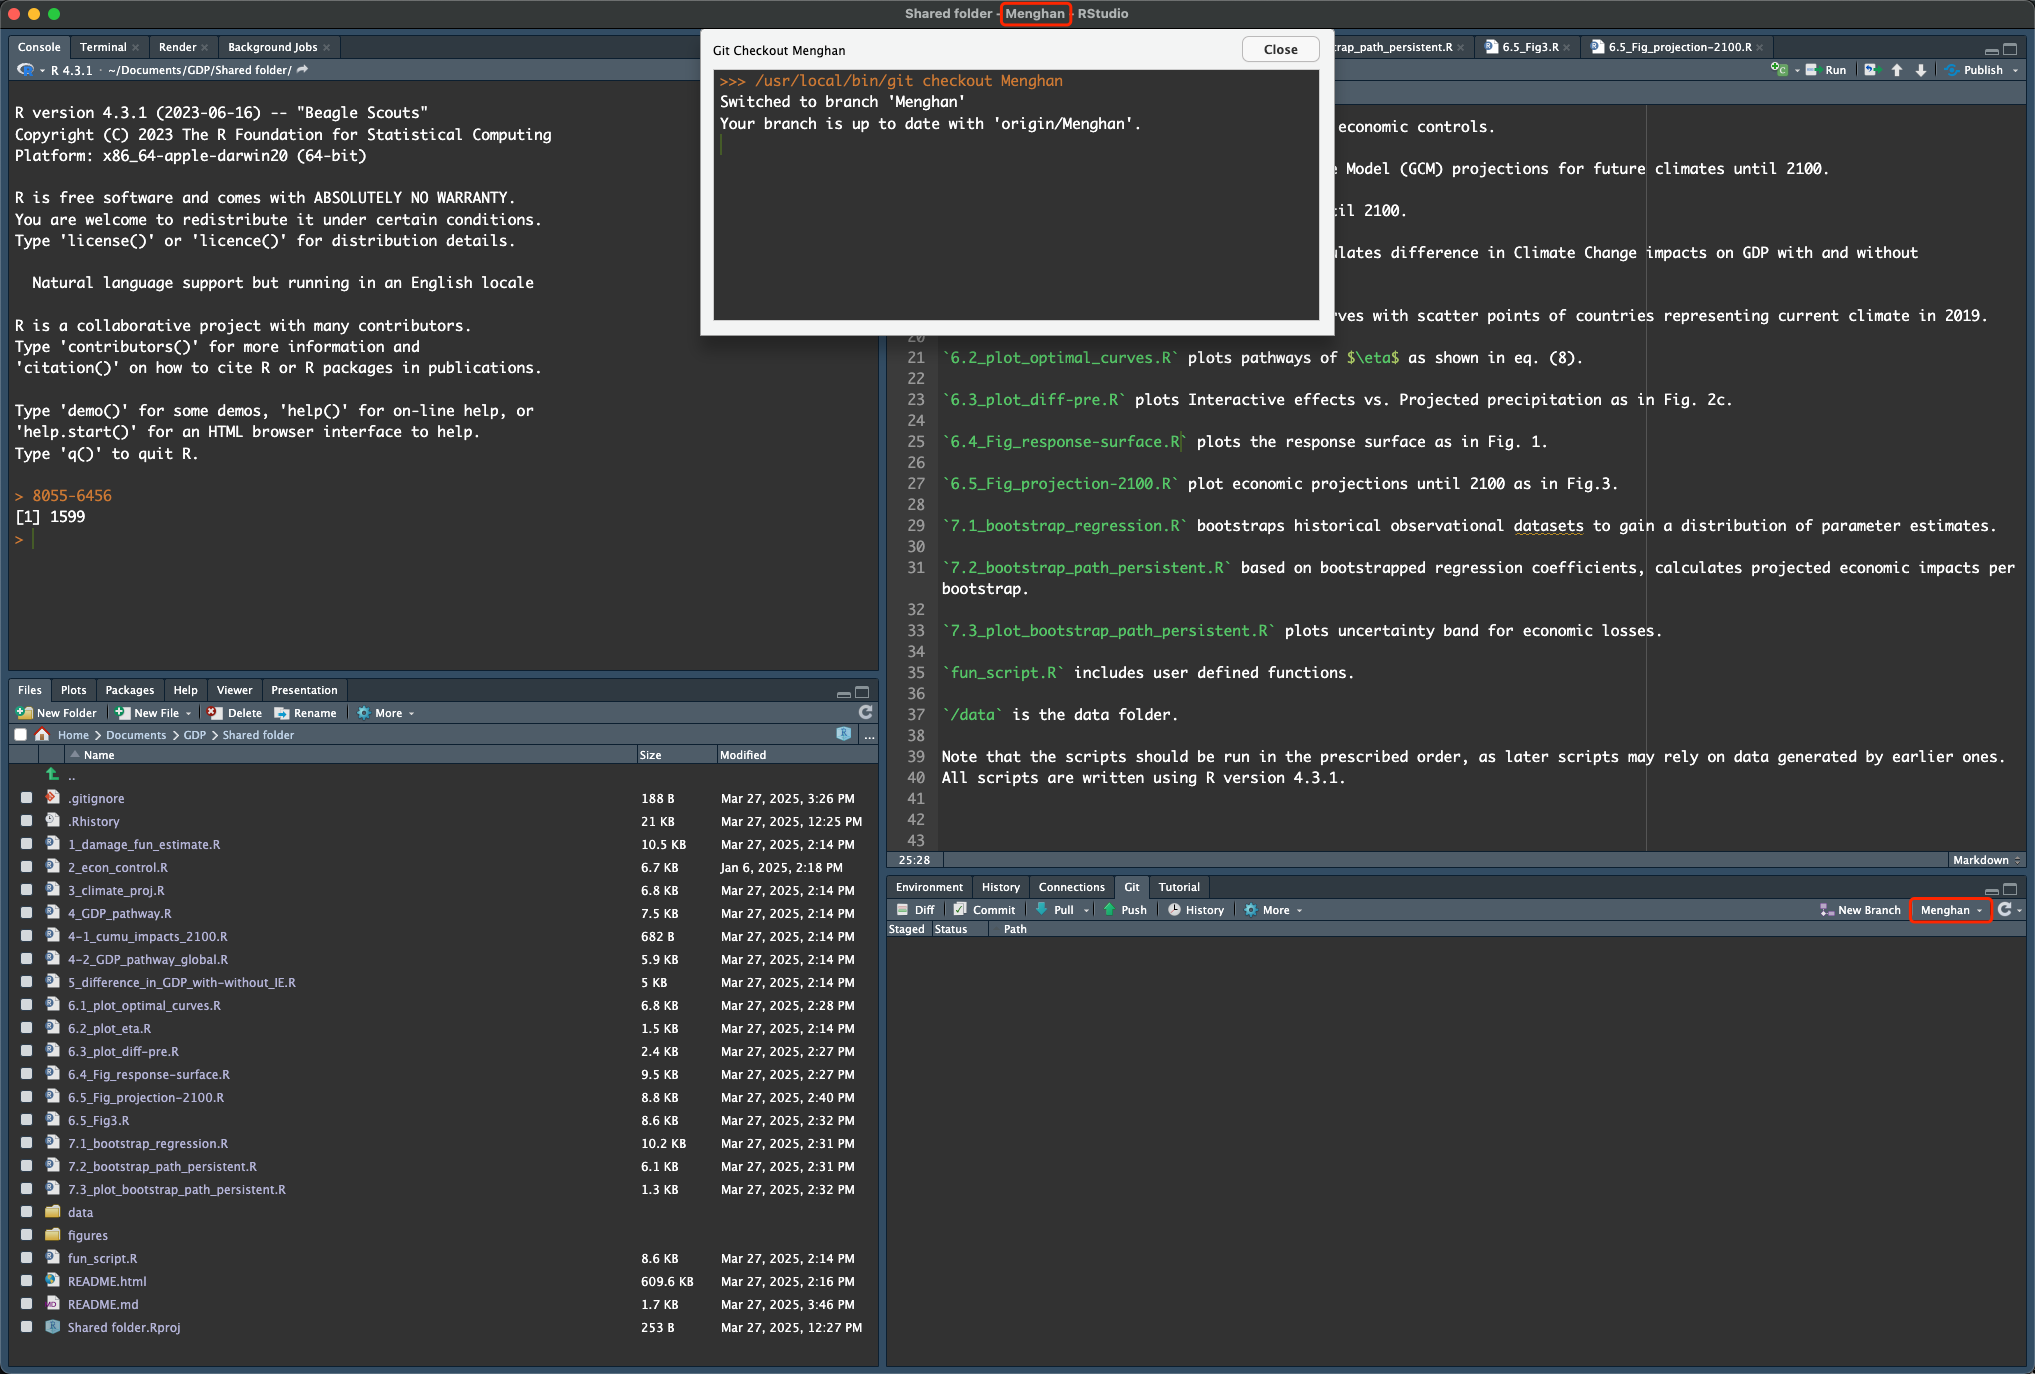
\includegraphics[width=1\linewidth]{images/R git branch}

\chapter{Knit Rmd}\label{knit-rmd}

R Markdown is a powerful tool for combining analysis and reporting into the same document. R Markdown has grown substantially from a package that supports a few output formats, to an extensive and diverse ecosystem that supports the creation of books, blogs, scientific articles, websites, and even resumes.

Nice documentations

\begin{itemize}
\tightlist
\item
  \href{https://bookdown.org/yihui/rmarkdown}{R markdown: The definitive guide.} provides detailed references
\item
  \href{https://bookdown.org/yihui/rmarkdown-cookbook/}{R markdown cookbook} concise and covers essential functions, with examples.
\end{itemize}

\textbf{Quick takeaways}:

\begin{itemize}
\tightlist
\item
  Can still use horizontal separator ctrl + shift + S for dashed lines and ctrl + shift + = for equals
\item
  Headers must have one empty line above and below to separate it from other text
\end{itemize}

\textbf{YAML metadata}

Q: What is YAML?

A: YAML is a human-friendly data serialization language for all programming languages.

Q: What does YAML do?

A: It is placed at the very beginning of the document and is read by each of Pandoc, \textbf{rmarkdown}, and \textbf{knitr}.

\begin{itemize}
\tightlist
\item
  Provide metadata of the document.
\item
  located at the top of the file.
\item
  adheres to the YAML format and is delimited by lines containing three three dashes (\texttt{-\/-\/-}).
\end{itemize}

It can set values of the template variables, such as \texttt{title}, \texttt{author}, and \texttt{date} of the document.

\begin{itemize}
\item
  The \texttt{output} field is used by rmarkdown to apply the output format function \texttt{rmarkdown::html\_document()} in the rendering process.

  There are two types of output formats in the \textbf{rmarkdown} package: documents (e.g., \texttt{pdf\_document}), and presentations (e.g., \texttt{beamer\_presentation}).

  Supported output format examples: \texttt{html\_document}, \texttt{pdf\_document}.

  R Markdown documents (\texttt{html\_documents}) and R Notebook documents (\texttt{html\_notebook}) are very similar; in fact, an R Notebook document is a special type of R Markdown document. The main difference is using R Markdown document (\texttt{html\_documents}) you have to knit (render) the entire document each time you want to preview the document, even if you have made a minor change. However, using an R Notebook document (\texttt{html\_notebook}) you can view a preview of the final document without rendering the entire document.
\item
  Many aspects of the LaTeX template used to create PDF documents can be customized using \emph{top-level} \href{https://bookdown.org/yihui/rmarkdown/pdf-document.html\#tab:latex-vars}{YAML metadata} (note that these options do not appear underneath the \texttt{output} section, but rather appear at the top level along with \texttt{title}, \texttt{author}, and so on). For example:

\begin{Shaded}
\begin{Highlighting}[]
\SpecialCharTok{{-}{-}{-}}
\NormalTok{title}\SpecialCharTok{:} \StringTok{"Crop Analysis Q3 2013"}
\NormalTok{output}\SpecialCharTok{:}\NormalTok{ pdf\_document}
\NormalTok{fontsize}\SpecialCharTok{:} \DecValTok{11}\NormalTok{pt}
\NormalTok{geometry}\SpecialCharTok{:}\NormalTok{ margin}\OtherTok{=}\DecValTok{1}\DataTypeTok{i}\NormalTok{n}
\SpecialCharTok{{-}{-}{-}}
\end{Highlighting}
\end{Shaded}

  A few available metadata variables are displayed in the following (consult the Pandoc manual for \href{https://pandoc.org/MANUAL.html\#variables-for-latex}{the full list}):

  \begin{longtable}[]{@{}
    >{\raggedright\arraybackslash}p{(\linewidth - 2\tabcolsep) * \real{0.4340}}
    >{\raggedright\arraybackslash}p{(\linewidth - 2\tabcolsep) * \real{0.5660}}@{}}
  \toprule\noalign{}
  \begin{minipage}[b]{\linewidth}\raggedright
  Variable
  \end{minipage} & \begin{minipage}[b]{\linewidth}\raggedright
  Description
  \end{minipage} \\
  \midrule\noalign{}
  \endhead
  \bottomrule\noalign{}
  \endlastfoot
  \texttt{lang} & Document language code \\
  \texttt{fontsize} & Font size (e.g., \texttt{10pt}, \texttt{11pt}, or \texttt{12pt}) \\
  \texttt{documentclass} & LaTeX document class (e.g., \texttt{article}) \\
  \texttt{classoption} & Options for documentclass (e.g., \texttt{oneside}) \\
  \texttt{geometry} & Options for geometry class (e.g., \texttt{margin=1in}) \\
  \texttt{mainfont}, \texttt{sansfont}, \texttt{monofont}, \texttt{mathfont} & Document fonts (works only with \texttt{xelatex} and \texttt{lualatex}) \\
  \texttt{linkcolor}, \texttt{urlcolor}, \texttt{citecolor} & Color for internal links (cross references), external links (link to websites), and citation links (bibliography) \\
  \texttt{linestretch} & Options for line spacing (e.g.~1, 1.5, 3). \\
  \end{longtable}

  \begin{itemize}
  \item
    In PDFs, you can use code, typesetting commands (e.g., \texttt{\textbackslash{}vspace\{12pt\}}), and specific packages from LaTeX.

    \begin{enumerate}
    \def\labelenumi{\arabic{enumi}.}
    \tightlist
    \item
      The \texttt{header-includes} option loads LaTeX packages.
    \end{enumerate}

\begin{Shaded}
\begin{Highlighting}[]
\SpecialCharTok{{-}{-}{-}}
\NormalTok{output}\SpecialCharTok{:}\NormalTok{ pdf\_document}
\NormalTok{header}\SpecialCharTok{{-}}\NormalTok{includes}\SpecialCharTok{:}
\SpecialCharTok{{-}}\NormalTok{ \textbackslash{}usepackage\{fancyhdr\}}
\SpecialCharTok{{-}{-}{-}}

\NormalTok{\textbackslash{}pagestyle\{fancy\}}
\NormalTok{\textbackslash{}fancyhead[LE,RO]\{Holly Zaharchuk\}}
\NormalTok{\textbackslash{}fancyhead[LO,RE]\{PSY }\DecValTok{508}\NormalTok{\}}

\CommentTok{\# Problem Set 12}
\end{Highlighting}
\end{Shaded}

    \begin{enumerate}
    \def\labelenumi{\arabic{enumi}.}
    \setcounter{enumi}{1}
    \tightlist
    \item
      Alternatively, use \texttt{extra\_dependencies} to list a character vector of LaTeX packages. This is useful if you need to load multiple packages:
    \end{enumerate}

\begin{Shaded}
\begin{Highlighting}[]
\SpecialCharTok{{-}{-}{-}}
\NormalTok{title}\SpecialCharTok{:} \StringTok{"Untitled"}
\NormalTok{output}\SpecialCharTok{:} 
\NormalTok{  pdf\_document}\SpecialCharTok{:}
\NormalTok{    extra\_dependencies}\SpecialCharTok{:}\NormalTok{ [}\StringTok{"bbm"}\NormalTok{, }\StringTok{"threeparttable"}\NormalTok{]}
\SpecialCharTok{{-}{-}{-}}
\end{Highlighting}
\end{Shaded}

    f you need to specify options when loading the package, you can add a second-level to the list and provide the options as a list:

\begin{Shaded}
\begin{Highlighting}[]
\SpecialCharTok{{-}{-}{-}}
\NormalTok{title}\SpecialCharTok{:} \StringTok{"Untitled"}
\NormalTok{output}\SpecialCharTok{:} 
\NormalTok{  pdf\_document}\SpecialCharTok{:}
\NormalTok{    extra\_dependencies}\SpecialCharTok{:}
\NormalTok{      caption}\SpecialCharTok{:}\NormalTok{ [}\StringTok{"labelfont=\{bf\}"}\NormalTok{]}
\NormalTok{      hyperref}\SpecialCharTok{:}\NormalTok{ [}\StringTok{"unicode=true"}\NormalTok{, }\StringTok{"breaklinks=true"}\NormalTok{]}
\NormalTok{      lmodern}\SpecialCharTok{:}\NormalTok{ null}
\SpecialCharTok{{-}{-}{-}}
\end{Highlighting}
\end{Shaded}

    Here are some examples of LaTeX packages you could consider using within your report:

    \begin{itemize}
    \tightlist
    \item
      \href{https://ctan.org/pkg/pdfpages}{pdfpages}: Include full PDF pages from an external PDF document within your document.
    \item
      \href{https://ctan.org/pkg/caption}{caption}: Change the appearance of caption subtitles. For example, you can make the figure title italic or bold.
    \item
      \href{https://ctan.org/pkg/fancyhdr}{fancyhdr}: Change the style of running headers of all pages.
    \end{itemize}
  \item
    Some options are passed to Pandoc, such as \texttt{toc}, \texttt{toc\_depth}, and \texttt{number\_sections}. You should consult the \href{https://pandoc.org/MANUAL.html\#variables}{Pandoc documentation} when in doubt.

\begin{Shaded}
\begin{Highlighting}[]
\SpecialCharTok{{-}{-}{-}}
\NormalTok{output}\SpecialCharTok{:}
\NormalTok{  pdf\_document}\SpecialCharTok{:}
\NormalTok{    toc}\SpecialCharTok{:}\NormalTok{ true}
\NormalTok{        keep\_tex}\SpecialCharTok{:}\NormalTok{ true}
\SpecialCharTok{{-}{-}{-}}
\end{Highlighting}
\end{Shaded}

    \begin{itemize}
    \tightlist
    \item
      \texttt{keep\_tex:\ true} if you want to keep intermediate TeX. Easy to debug. Defaults to \texttt{false}.
    \end{itemize}
  \end{itemize}
\end{itemize}

We can include variables and R expressions in this header that can be referenced throughout our R Markdown document. For example, the following header defines \texttt{start\_date} and \texttt{end\_date} parameters, which will be reflected in a list called \texttt{params} later in the R Markdown document.

Thus, if we want to use these values in our R code, we can access them via \texttt{params\$start\_date} and \texttt{params\$end\_date}.

Should I use quotes to surround the values?

\begin{itemize}
\tightlist
\item
  Whenever applicable use the unquoted style since it is the most readable.
\item
  Use quotes when the value can be misinterpreted as a data type or the value contains a \texttt{:}.
\end{itemize}

\begin{Shaded}
\begin{Highlighting}[]
\CommentTok{\# values need quotes}
\NormalTok{foo}\SpecialCharTok{:} \StringTok{\textquotesingle{}\{\{ bar \}\}\textquotesingle{}} \CommentTok{\# need quotes to avoid interpreting as \textasciigrave{}dict\textasciigrave{} object}
\NormalTok{foo}\SpecialCharTok{:} \StringTok{\textquotesingle{}123\textquotesingle{}}       \CommentTok{\# need quote to avoid interpreting as \textasciigrave{}int\textasciigrave{} object}
\NormalTok{foo}\SpecialCharTok{:} \StringTok{\textquotesingle{}yes\textquotesingle{}}           \CommentTok{\# avoid interpreting as \textasciigrave{}boolean\textasciigrave{} object}
\NormalTok{foo}\SpecialCharTok{:} \StringTok{"bar:baz:bam"} \CommentTok{\# has colon, can be misinterpreted as key}

\CommentTok{\# values need not quotes}
\NormalTok{foo}\SpecialCharTok{:}\NormalTok{ bar1baz234}
\NormalTok{bar}\SpecialCharTok{:} \DecValTok{123}\NormalTok{baz}
\end{Highlighting}
\end{Shaded}

\section{Chunk Options}\label{chunk-options}

If you want to set chunk options globally, call \texttt{knitr::opts\_chunk\$set()} in a code chunk (usually the first one in the document), e.g.,

\begin{Shaded}
\begin{Highlighting}[]
\InformationTok{\textasciigrave{}\textasciigrave{}\textasciigrave{}\{r, label="setup", include=FALSE\}}
\InformationTok{knitr::opts\_chunk$set(}
\InformationTok{  comment = "\#\textgreater{}", echo = FALSE, fig.width = 6}
\InformationTok{)}
\InformationTok{\textasciigrave{}\textasciigrave{}\textasciigrave{}}
\end{Highlighting}
\end{Shaded}

Full list of chunk options: \url{https://yihui.org/knitr/options/}

Chunk options can customize nearly all components of code chunks, such as the source code, text output, plots, and the language of the chunk.

\textbf{Other languages are supported in \texttt{Rmd}}

You can list the names of all available engines via:

\begin{Shaded}
\begin{Highlighting}[]
\FunctionTok{names}\NormalTok{(knitr}\SpecialCharTok{::}\NormalTok{knit\_engines}\SpecialCharTok{$}\FunctionTok{get}\NormalTok{())}
\DocumentationTok{\#\#  [1] "awk"          "bash"         "coffee"      }
\DocumentationTok{\#\#  [4] "gawk"         "groovy"       "haskell"     }
\DocumentationTok{\#\#  [7] "lein"         "mysql"        "node"        }
\DocumentationTok{\#\# [10] "octave"       "perl"         "php"         }
\DocumentationTok{\#\# [13] "psql"         "Rscript"      "ruby"        }
\DocumentationTok{\#\# [16] "sas"          "scala"        "sed"         }
\DocumentationTok{\#\# [19] "sh"           "stata"        "zsh"         }
\DocumentationTok{\#\# [22] "asis"         "asy"          "block"       }
\DocumentationTok{\#\# [25] "block2"       "bslib"        "c"           }
\DocumentationTok{\#\# [28] "cat"          "cc"           "comment"     }
\DocumentationTok{\#\# [31] "css"          "ditaa"        "dot"         }
\DocumentationTok{\#\# [34] "embed"        "eviews"       "exec"        }
\DocumentationTok{\#\# [37] "fortran"      "fortran95"    "go"          }
\DocumentationTok{\#\# [40] "highlight"    "js"           "julia"       }
\DocumentationTok{\#\# [43] "python"       "R"            "Rcpp"        }
\DocumentationTok{\#\# [46] "sass"         "scss"         "sql"         }
\DocumentationTok{\#\# [49] "stan"         "targets"      "tikz"        }
\DocumentationTok{\#\# [52] "verbatim"     "theorem"      "lemma"       }
\DocumentationTok{\#\# [55] "corollary"    "proposition"  "conjecture"  }
\DocumentationTok{\#\# [58] "definition"   "example"      "exercise"    }
\DocumentationTok{\#\# [61] "hypothesis"   "proof"        "remark"      }
\DocumentationTok{\#\# [64] "solution"     "marginfigure"}
\end{Highlighting}
\end{Shaded}

The engines from \texttt{theorem} to \texttt{solution} are only available when you use the \textbf{bookdown} package, and the rest are shipped with the \textbf{knitr} package.

To use a different language engine, you can change the language name in the chunk header from \texttt{r} to the engine name, e.g.,

\begin{Shaded}
\begin{Highlighting}[]
\StringTok{\textasciigrave{}\textasciigrave{}\textasciigrave{}}\AttributeTok{python}
\AttributeTok{x = \textquotesingle{}hello, python world!\textquotesingle{}}
\AttributeTok{print(x.split(\textquotesingle{} \textquotesingle{}))}
\StringTok{\textasciigrave{}\textasciigrave{}\textasciigrave{}}
\end{Highlighting}
\end{Shaded}

For engines that rely on external interpreters such as \texttt{python}, \texttt{perl}, and \texttt{ruby}, the default interpreters are obtained from \texttt{Sys.which()}, i.e., using the interpreter found via the environment variable \texttt{PATH} of the system. If you want to use an alternative interpreter, you may specify its path in the chunk option \texttt{engine.path}.

For example, you may want to use Python 3 instead of the default Python 2, and we assume Python 3 is at \texttt{/usr/bin/python3}

\begin{Shaded}
\begin{Highlighting}[]
\InformationTok{\textasciigrave{}\textasciigrave{}\textasciigrave{}\{python, engine.path = \textquotesingle{}/usr/bin/python3\textquotesingle{}\}}
\InformationTok{import sys}
\InformationTok{print(sys.version)}
\InformationTok{\textasciigrave{}\textasciigrave{}\textasciigrave{}}
\end{Highlighting}
\end{Shaded}

\begin{itemize}
\tightlist
\item
  All outputs support markdown syntax.
\item
  If the output is html, you can write in html syntax.
\end{itemize}

The \textbf{chunk label} for each chunk is assumed to be unique within the document. This is especially important for cache and plot filenames, because these filenames are based on chunk labels. Chunks without labels will be assigned labels like \texttt{unnamed-chunk-i}, where \texttt{i} is an incremental number.

\begin{itemize}
\item
  Chunk label doesn't need a \texttt{tag}, i.e., you only provide the \texttt{value}.
\item
  If you prefer the form \texttt{tag=value}, you could also use the chunk option \texttt{label} explicitly, e.g.,

\begin{Shaded}
\begin{Highlighting}[]
\InformationTok{\textasciigrave{}\textasciigrave{}\textasciigrave{}\{r, label=\textquotesingle{}my{-}chunk\textquotesingle{}\}}
\InformationTok{\# one code chunk example}
\InformationTok{\textasciigrave{}\textasciigrave{}\textasciigrave{}}
\end{Highlighting}
\end{Shaded}
\end{itemize}

You may use \texttt{knitr::opts\_chunk\$set()} to change the default values of chunk options in a document.

\textbf{Commonly used chunk options}

\begin{itemize}
\tightlist
\item
  Complete list \href{https://yihui.org/knitr/options/}{here}. Or \texttt{?opts\_chunk} to get the help page.
\end{itemize}

\begin{longtable}[]{@{}
  >{\raggedright\arraybackslash}p{(\linewidth - 2\tabcolsep) * \real{0.2500}}
  >{\raggedright\arraybackslash}p{(\linewidth - 2\tabcolsep) * \real{0.7500}}@{}}
\toprule\noalign{}
\begin{minipage}[b]{\linewidth}\raggedright
Options
\end{minipage} & \begin{minipage}[b]{\linewidth}\raggedright
Definitions
\end{minipage} \\
\midrule\noalign{}
\endhead
\bottomrule\noalign{}
\endlastfoot
\texttt{echo=TRUE} & Whether to display the \textbf{source code} in the output document.Use this when you want to show the output but not the code itself. \\
\texttt{eval=TRUE} & Whether to evaluate the code chunk. \\
\texttt{include=TRUE} & Whether to include the {chunk \textbf{output}} in the output document. If \texttt{FALSE}, nothing will be written into the output document, but the code is still evaluated and plot files are generated if there are any plots in the chunk, so you can manually insert figures later. \\
\texttt{message=TRUE} & Whether to preserve messages emitted by \texttt{message()} \\
\texttt{warning=TRUE} & Whether to show warnings in the output produced by \texttt{warning()}. \\
\texttt{results=\textquotesingle{}markup\textquotesingle{}} & Controls how to display the text results. When \texttt{results=\textquotesingle{}markup\textquotesingle{}} that is to write text output as-is, i.e., write the raw text results directly into the output document without any markups.Useful when priting \texttt{stargazer} tables. \\
\texttt{comment=\textquotesingle{}\#\#\textquotesingle{}} & The prefix to be added before each line of the text output. Set \texttt{comment\ =\ \textquotesingle{}\textquotesingle{}} remove the default \texttt{\#\#}. \\
\texttt{fig.keep=\textquotesingle{}high\textquotesingle{}} & How plots in chunks should be kept. \texttt{high}: Only keep high-level plots (merge low-level changes into high-level plots). \texttt{none}: Discard all plots. \texttt{all}: Keep all plots (low-level plot changes may produce new plots). \texttt{first}: Only keep the first plot. \texttt{last}: Only keep the last plot. If set to a numeric vector, the values are indices of (low-level) plots to keep.If you want to choose the second to the fourth plots, you could use \texttt{fig.keep\ =\ 2:4} (or remove the first plot via \texttt{fig.keep\ =\ -1}). \\
\texttt{fig.align="center"} & Figure alignment. \\
\texttt{fig.pos="H"} & A character string for the figure position arrangement to be used in \texttt{\textbackslash{}begin\{figure\}{[}{]}}. \\
\texttt{fig.cap} & Figure caption. \\
\end{longtable}

{\texttt{results=\textquotesingle{}markup\textquotesingle{}}} note plural form for result\textbf{s}.

\begin{itemize}
\item
  \texttt{markup}: Default. Mark up text output with the appropriate environments depending on the output format. For example, for R Markdown, if the text output is a character string \texttt{"{[}1{]}\ 1\ 2\ 3"}, the actual output that \textbf{knitr} produces will be:

\begin{Shaded}
\begin{Highlighting}[]
\StringTok{\textasciigrave{}\textasciigrave{}\textasciigrave{}}
\AttributeTok{[1] 1 2 3}
\StringTok{\textasciigrave{}\textasciigrave{}\textasciigrave{}}
\end{Highlighting}
\end{Shaded}

  In this case, \texttt{results=\textquotesingle{}markup\textquotesingle{}} means to put the text output in fenced code blocks (```).
\item
  \texttt{asis}: Write text output as-is, i.e., write the raw text results directly into the output document without any markups.

\begin{Shaded}
\begin{Highlighting}[]
\InformationTok{\textasciigrave{}\textasciigrave{}\textasciigrave{}\{r, results=\textquotesingle{}asis\textquotesingle{}\}}
\InformationTok{cat("I\textquotesingle{}m raw **Markdown** content.\textbackslash{}n")}
\InformationTok{\textasciigrave{}\textasciigrave{}\textasciigrave{}}
\end{Highlighting}
\end{Shaded}

  Sometime, you encounter the following error messages when you have R codes within \texttt{enumerate} environment.

  \begin{quote}
  You can't use \texttt{macro\ parameter\ character\ \#} in horizontal mode.
  \end{quote}

  By default, knitr prefixes R output with \texttt{\#\#}, which can't be present in your TeX file.

  Solution:

  \begin{itemize}
  \tightlist
  \item
    specify \texttt{results="asis"} in code chunks.
  \end{itemize}
\item
  \texttt{hold}: Hold all pieces of text output in a chunk and flush them to the end of the chunk.
\item
  \texttt{hide} (or \texttt{FALSE}): Hide text output.
\end{itemize}

\begin{center}\rule{0.5\linewidth}{0.5pt}\end{center}

\section{Print Verbatim R code chunks}\label{print-verbatim-r-code-chunks}

\textbf{Including verbatim R code chunks inside R Markdown}

One solution for including verbatim R code chunks (see below for more) is to insert hidden inline R code (\texttt{\textasciigrave{}r\ \ \ \textquotesingle{}\textquotesingle{}\textasciigrave{}}) immediately before or after your R code chunk.

\begin{itemize}
\tightlist
\item
  The hidden inline R code will be evaluated as an inline expression to an empty string by knitr.
\end{itemize}

Then wrap the whole block within a markdown code block. The rendered output will display the verbatim R code chunk --- including backticks.

R code generating the four backticks block:

\begin{Shaded}
\begin{Highlighting}[]
\NormalTok{output\_code }\OtherTok{\textless{}{-}}
\StringTok{"\textasciigrave{}\textasciigrave{}\textasciigrave{}\textasciigrave{}markdown}
\StringTok{\textasciigrave{}\textasciigrave{}\textasciigrave{}\{r\}}
\StringTok{plot(cars)}
\StringTok{\textasciigrave{}\textasciigrave{}\textasciigrave{} }\SpecialCharTok{\textbackslash{}n}\StringTok{\textasciigrave{}\textasciigrave{}\textasciigrave{}\textasciigrave{}"}
\FunctionTok{cat}\NormalTok{(output\_code)}
\end{Highlighting}
\end{Shaded}

Write this code in your R Markdown document:

\begin{verbatim}
````markdown
`r ''````{r}
plot(cars)
``` 
````
\end{verbatim}

or

\begin{verbatim}
````markdown
```{r}`r ''`
plot(cars)
``` 
````
\end{verbatim}

Knit the document and the code will render like this in your output:

\begin{Shaded}
\begin{Highlighting}[]
\InformationTok{\textasciigrave{}\textasciigrave{}\textasciigrave{}\{r\}}
\InformationTok{plot(cars)}
\InformationTok{\textasciigrave{}\textasciigrave{}\textasciigrave{}}
\end{Highlighting}
\end{Shaded}

\textbf{References}:

\url{https://yihui.org/en/2017/11/knitr-verbatim-code-chunk/}

\url{https://support.posit.co/hc/en-us/articles/360018181633-Including-verbatim-R-code-chunks-inside-R-Markdown}

\url{https://themockup.blog/posts/2021-08-27-displaying-verbatim-code-chunks-in-xaringan-presentations/}

\chapter{Machine Learning}\label{machine-learning}

Parametric models such as generalized linear regression and logistic regression has advantages and disadvantages.

\textbf{Strength}:

\begin{itemize}
\tightlist
\item
  The effects of individual predictors on the outcome are easily understood
\item
  Statistical inference, such as hypothesis testing or interval estimation, is straightforward
\item
  Methods and procedures for selecting, comparing, and summarizing these models are well-established and extensively studied
\end{itemize}

\textbf{Disadvantages} in the following scenarios:

\begin{itemize}
\tightlist
\item
  Complex, non-linear relationships between predictors and the outcome
\item
  High degrees of interaction between predictors
\item
  Nominal outcome variables with several categories
\end{itemize}

In these situations, non-parametric or algorithmic modeling approaches have the potential to better capture the underlying trends in the data.

Here we introduce three models: classification and regression trees (CART), random forests, k-nearest neighbors.

\begin{itemize}
\item
  Classification and regression trees (CART) are ``trained'' by recursively partitioning the 𝑝-dimensional space (defined by the explanatory variables) until an acceptable level of homogeneity or ``purity'' is achieved within each partition.
\item
  A major issue with tree-based models is that they tend to be high variance (leading to a high propensity towards over-fitting). Random forests are a non-parametric, tree-based modeling algorithm that is built upon the idea that averaging a set of independent elements yields an outcome with lower variability than any of the individual elements in the set.

  This general concept should seem familiar. Thinking back to your introductory statistics course, you should remember that the sample mean, \(\overline{x}\), of a dataset has substantially less variability (\(\frac{\sigma}{\sqrt{n}}\)) than the individual data-points themselves (\(\sigma\)).
\end{itemize}

Q: What is Bias-Variance Trade-Off in Machine Learning?\\
A:

\begin{itemize}
\tightlist
\item
  Bias refers to error caused by a model for solving complex problems that is over simplified, makes significant assumptions, and misses important relationships in your data.
\item
  Variance error is variability of a target function's form with respect to different training sets. Models with small variance error will not change much if you replace couple of samples in training set. Models with high variance might be affected even with small changes in training set. High variance models fit the data too well, and learns the noise in addition to the inherent patterns in the data.
\end{itemize}

\section{Random Forest}\label{random-forest}

\textbf{Averaging of independent trees}

The goal of bagging is to produce \(\boldsymbol{B}\) separate training datasets that are independent of each other (typically 𝐵 is in the hundreds). The model of interest (in this case classification and regression trees) is trained separately on each of these datasets, resulting in \(\boldsymbol{B}\) different estimated ``models''. These are then averaged to produce a single, low-variance estimate.

Bagging is a general approach, but its most well-known application is in the random forest algorithm:

\begin{enumerate}
\def\labelenumi{\arabic{enumi}.}
\tightlist
\item
  Construct \(\boldsymbol{B}\) bootstrap samples by sampling cases from the original dataset with replacement (this results in \(\boldsymbol{B}\) unique datasets that are similar to the original)
\item
  Fit a classification and regression tree to each sample, but randomly choose a subset of \(m\) variables that can be used in the construction of that tree (this results in \(\boldsymbol{B}\) unique trees that are fit to similar datasets using different sets of predictors)
\item
  For a given data-point, each of the \(\boldsymbol{B}\) trees in the forest contributes a prediction or ``vote'', with the majority (or average) of these votes forming the random forest's final prediction, \(\hat{y}_i\)
\end{enumerate}

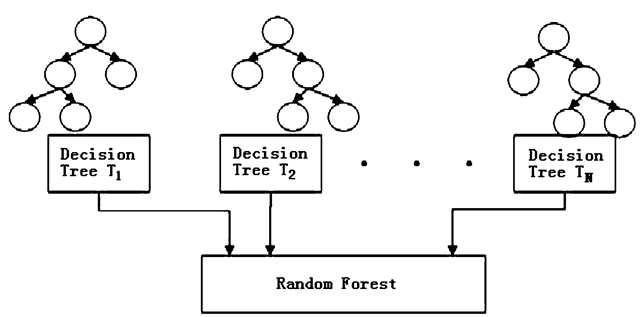
\includegraphics[width=0.8\linewidth]{images/rf}

A downside of both the CART and random forest algorithms (as well as many other algorithmic modeling approaches) is an inability to clearly quantify the roles played by individual variables in making predictions. However, the importance of individual variables in a random forest can still be expressed using a measure known as variable importance.

The random forest algorithm requires the following tuning parameters be specified in order to run:

\begin{itemize}
\tightlist
\item
  \texttt{ntree} - the number of bagged samples, \(\boldsymbol{B}\), onto which trees will be grown
\item
  \texttt{mtry} - the number of variables that are randomly chosen to be candidates at each split
\item
  Some sort of stopping criteria for individual trees, this can be:

  \begin{itemize}
  \tightlist
  \item
    \texttt{nodesize}, which sets the minimum size of terminal nodes

    \begin{itemize}
    \tightlist
    \item
      larger \texttt{nodesize} leads to shallower trees
    \item
      smaller node size allows for deeper, more complex trees
    \end{itemize}
  \item
    \texttt{maxnodes}, which sets the maximum number of terminal nodes an individual tree can have.
  \end{itemize}
\end{itemize}

\textbf{Applications of Random Forest}

Some of the applications of Random Forest Algorithm are listed below:

\begin{itemize}
\tightlist
\item
  Banking: It predicts a loan applicant's solvency. This helps lending institutions make a good decision on whether to give the customer loan or not. They are also being used to detect fraudsters.
\item
  Health Care: Health professionals use random forest systems to diagnose patients. Patients are diagnosed by assessing their previous medical history. Past medical records are reviewed to establish the proper dosage for the patients.
\item
  Stock Market: Financial analysts use it to identify potential markets for stocks. It also enables them to remember the behaviour of stocks.
\item
  E-Commerce: Through this system, e-commerce vendors can predict the preference of customers based on past consumption behaviour.
\end{itemize}

\textbf{When to Avoid Using Random Forests?}

Random Forests Algorithms are not ideal in the following situations:

\begin{itemize}
\tightlist
\item
  Extrapolation: Random Forest regression is not ideal in the extrapolation of data. Unlike linear regression, which uses existing observations to estimate values beyond the observation range.
\item
  Sparse Data: Random Forest does not produce good results when the data is sparse. In this case, the subject of features and bootstrapped sample will have an invariant space. This will lead to unproductive spills, which will affect the outcome.
\end{itemize}

\textbf{FAQ}

Q: Is RF a linear or non-linear model?\\
A: RF can capture complex, non-linear relationships.

Q: Is RF sensitive to Imbalanced Data?\\
A: Yes. It may perform poorly if the dataset is highly imbalanced like one class is significantly more frequent than another.

Q: What is the loss function?\\
A: Entropy/gini or any other loss function you want.

Q: Difference btw RF and a linear model?\\
A: A major difference is that a decision tree does not have ``parameters'', whereas the linear models need to create a functional form and find the optimal parameters.

\begin{center}\rule{0.5\linewidth}{0.5pt}\end{center}

\subsection*{Implementation in R}\label{implementation-in-r}
\addcontentsline{toc}{subsection}{Implementation in R}

\texttt{ranger} package offers a computation efficient function for RF.

\begin{Shaded}
\begin{Highlighting}[]
\NormalTok{RF\_ranger }\OtherTok{\textless{}{-}} \FunctionTok{ranger}\NormalTok{(}\AttributeTok{formula =}\NormalTok{ formula, }
                    \AttributeTok{data =}\NormalTok{ data\_before[idx,], }
                    \AttributeTok{probability =} \ConstantTok{TRUE}\NormalTok{,}
                    \AttributeTok{importance =} \StringTok{"permutation"}\NormalTok{, }
                    \AttributeTok{scale.permutation.importance =} \ConstantTok{TRUE}\NormalTok{,}
\NormalTok{                    )}
    \CommentTok{\# print(RF\_ranger)}
    
\NormalTok{rf.pred.test }\OtherTok{\textless{}{-}} \FunctionTok{predict}\NormalTok{(RF\_ranger, }\AttributeTok{data=}\NormalTok{data\_before[}\SpecialCharTok{{-}}\NormalTok{idx,])}\SpecialCharTok{$}\NormalTok{predictions}
\end{Highlighting}
\end{Shaded}

Parameters controlling the general process of RF:

\begin{itemize}
\tightlist
\item
  \texttt{probability=FALSE}: Whether to forecast a probability forest.
\end{itemize}

The hyperparameters \texttt{mtry}, \texttt{min.node.size} and \texttt{sample.fraction} determine the degree of randomness, and should be tuned.

\begin{itemize}
\tightlist
\item
  \texttt{mtry=500}: Number of variables to possibly split at in each node in one tree. In plain language, it indicates how many predictor variables should be used in each tree.

  \begin{itemize}
  \tightlist
  \item
    Default is the (rounded down) square root of the number variables. Alternatively, a single argument function returning an integer, given the number of independent variables.
  \item
    Range btw 1 to the number of predictors.
  \item
    If all predictors are used, then this corresponds in fact to bagging.
  \end{itemize}
\item
  \texttt{min.node.size}: The number of observations a terminal node should at least have.

  \begin{itemize}
  \tightlist
  \item
    Default 1 for classification, 5 for regression, 3 for survival, and 10 for probability. For classification, this can be a vector of class-specific values.
  \item
    Range between 1 and 10
  \end{itemize}
\item
  \texttt{sample.fraction}: Fraction of observations to be used in each tree. Default is 1 for sampling with replacement and 0.632 for sampling without replacement. For classification, this can be a vector of class-specific values.

  \begin{itemize}
  \tightlist
  \item
    Smaller fractions lead to greater diversity, and thus less correlated trees which often is desirable.
  \item
    Range between 0.2 and 0.9
  \end{itemize}
\end{itemize}

Parameters controlling what and how intermediate results are saved:

\begin{itemize}
\item
  \texttt{keep.inbag\ =\ FALSE}: Whether to save how often observations are in-bag in each tree.

  Set to \texttt{TRUE} if you want to check sample composition in each tree.
\item
  \texttt{importance\ =\ \textquotesingle{}none\textquotesingle{}\textbar{}\textquotesingle{}impurity\textquotesingle{}\textbar{}\textquotesingle{}impurity\_corrected\textquotesingle{}\textbar{}\textquotesingle{}permutation\textquotesingle{}}: Variable importance mode.
\item
  \texttt{scale.permutation.importance\ =\ FALSE}: Whether to scale permutation importance by standard error as in (Breiman 2001). Only applicable if \texttt{\textquotesingle{}permutation\textquotesingle{}} variable importance mode selected.
\item
  \texttt{write.forest\ =\ TRUE}: Whether to save \texttt{ranger.forest} object, required for prediction. Set to \texttt{FALSE} to reduce memory usage if no prediction intended.

  \begin{itemize}
  \tightlist
  \item
    Set to \texttt{FALSE} when you do parameter tuning.
  \end{itemize}
\end{itemize}

Q: How to tune hyperparameters?\\
A: Check out \href{https://mlr3.mlr-org.com}{\texttt{mlr3} package}. \href{https://r.geocompx.org/eco.html}{Here} is an example.

\begin{center}\rule{0.5\linewidth}{0.5pt}\end{center}

\subsection*{Imbalance Classification}\label{imbalance-classification}
\addcontentsline{toc}{subsection}{Imbalance Classification}

You can balance your random forests using case weights. Here's a simple example:

\begin{Shaded}
\begin{Highlighting}[]
\FunctionTok{library}\NormalTok{(ranger)}

\CommentTok{\# Make a dataste}
\FunctionTok{set.seed}\NormalTok{(}\DecValTok{43}\NormalTok{)}
\NormalTok{nrow }\OtherTok{\textless{}{-}} \DecValTok{1000}
\NormalTok{ncol }\OtherTok{\textless{}{-}} \DecValTok{10}
\NormalTok{X }\OtherTok{\textless{}{-}} \FunctionTok{matrix}\NormalTok{(}\FunctionTok{rnorm}\NormalTok{(nrow }\SpecialCharTok{*}\NormalTok{ ncol), }\AttributeTok{ncol=}\NormalTok{ncol)}
\NormalTok{CF }\OtherTok{\textless{}{-}} \FunctionTok{rnorm}\NormalTok{(ncol)}
\NormalTok{Y }\OtherTok{\textless{}{-}}\NormalTok{ (X }\SpecialCharTok{\%*\%}\NormalTok{ CF }\SpecialCharTok{+} \FunctionTok{rnorm}\NormalTok{(nrow))[,}\DecValTok{1}\NormalTok{]}
\NormalTok{Y }\OtherTok{\textless{}{-}} \FunctionTok{as.integer}\NormalTok{(Y }\SpecialCharTok{\textgreater{}} \FunctionTok{quantile}\NormalTok{(Y, }\FloatTok{0.90}\NormalTok{))}
\FunctionTok{table}\NormalTok{(Y)}

\CommentTok{\# Compute weights to balance the RF}
\NormalTok{w }\OtherTok{\textless{}{-}} \DecValTok{1}\SpecialCharTok{/}\FunctionTok{table}\NormalTok{(Y)}
\NormalTok{w }\OtherTok{\textless{}{-}}\NormalTok{ w}\SpecialCharTok{/}\FunctionTok{sum}\NormalTok{(w)}
\NormalTok{weights }\OtherTok{\textless{}{-}} \FunctionTok{rep}\NormalTok{(}\DecValTok{0}\NormalTok{, nrow)}
\NormalTok{weights[Y }\SpecialCharTok{==} \DecValTok{0}\NormalTok{] }\OtherTok{\textless{}{-}}\NormalTok{ w[}\StringTok{\textquotesingle{}0\textquotesingle{}}\NormalTok{]}
\NormalTok{weights[Y }\SpecialCharTok{==} \DecValTok{1}\NormalTok{] }\OtherTok{\textless{}{-}}\NormalTok{ w[}\StringTok{\textquotesingle{}1\textquotesingle{}}\NormalTok{]}
\FunctionTok{table}\NormalTok{(weights, Y)}

\CommentTok{\# Fit the RF}
\NormalTok{data }\OtherTok{\textless{}{-}} \FunctionTok{data.frame}\NormalTok{(}\AttributeTok{Y=}\FunctionTok{factor}\NormalTok{(}\FunctionTok{ifelse}\NormalTok{(Y}\SpecialCharTok{==}\DecValTok{0}\NormalTok{, }\StringTok{\textquotesingle{}no\textquotesingle{}}\NormalTok{, }\StringTok{\textquotesingle{}yes\textquotesingle{}}\NormalTok{)), X)}
\NormalTok{model }\OtherTok{\textless{}{-}} \FunctionTok{ranger}\NormalTok{(Y}\SpecialCharTok{\textasciitilde{}}\NormalTok{., data, }\AttributeTok{case.weights=}\NormalTok{weights)}
\FunctionTok{print}\NormalTok{(model)}
\end{Highlighting}
\end{Shaded}

Code Source: \url{https://stats.stackexchange.com/a/287849}

Fixed proportion sampling: \url{https://github.com/imbs-hl/ranger/issues/167}

\begin{center}\rule{0.5\linewidth}{0.5pt}\end{center}

\textbf{References}:

\url{https://remiller1450.github.io/m257s21/Lab10_Other_Models.html}

\section{Neural Network}\label{neural-network}

Neural networks are made up objects called ``layers'' and ``neurons'' and these things connect to each other in a specific way. Each layer has some number of neurons. For example, the first layer might have 10 neurons, the second might have 15, and so on. The number of layers and the number of neurons in each layer is a ``hyperparameter'', the user picks how many of each. Let's take a look at a single neuron.

\[
v_3^{(1)} = g(\boldsymbol{w}_3^{(1)}\boldsymbol{x} + b_3^{(1)})
\]

\begin{itemize}
\item
  The LHS, \(v_3^{(1)}\), will be the output. The superscript \((1)\) refers to the layer number; the subscript \(3\) refers to the neuron.

  An output here means just a single number. If we have say 15 neurons (subscript) for this first layer (superscript), then we will have 15 numbers come out of this first layer: \(\boldsymbol{v^{(1)}} = \{v^{(1)}_{1}, v^{(1)}_{1}, ..., v^{(1)}_{15}\}\) where the bolded \(v\) means a vector.
\item
  \(\boldsymbol{x}\) is our input vector.
\item
  \(\boldsymbol{w}\) is the weight/coefficient vector.
\item
  \(b\) is a bias or the intercept term, shifting the value of \(\boldsymbol{w}\cdot\boldsymbol{x}\) up or down.
\item
  \(g\) refers to a ``non-linear'' function, often called as the ``activation function''.
\end{itemize}

  \bibliography{book.bib,packages.bib}

\end{document}
